\documentclass[11pt,
			   %10pt, 
               %hyperref={colorlinks},
               aspectratio=169,
               hyperref={colorlinks}
               ]{beamer}
\usetheme{Singapore}
\usecolortheme[snowy, cautious]{owl}

\usepackage[utf8]{inputenc}
\usepackage[T1]{fontenc}
\usepackage[american]{babel}
\usepackage{graphicx}
\usepackage{hyperref}
\hypersetup{
    colorlinks=true,
    urlcolor=[rgb]{0,0,0.61},
    linkcolor=[rgb]{0,0,0.61}}

%------------------------------------------------------------------------------

\usepackage[natbib=true,style=numeric,backend=bibtex,useprefix=true]{biblatex}
%\setbeamercolor*{bibliography entry title}{fg=black}
%\setbeamercolor*{bibliography entry location}{fg=black}
%\setbeamercolor*{bibliography entry note}{fg=black}
\setbeamertemplate{bibliography item}{\insertbiblabel}
\setbeamerfont{caption}{size=\footnotesize}
\setbeamertemplate{frametitle continuation}{}

\definecolor{OwlGreen}{RGB}{51,0,102} % easier to see
\setcounter{tocdepth}{1}
\renewcommand*{\bibfont}{\scriptsize}
\addbibresource{lecture_4.bib}

\renewcommand*{\thefootnote}{\fnsymbol{footnote}}

\usenavigationsymbolstemplate{}
\setbeamertemplate{footline}{%
    \raisebox{5pt}{\makebox{\hfill\makebox[20pt]{\color{gray}
          \scriptsize\insertframenumber}}}\hspace*{5pt}}
          
          
\author{Patrick Hall}
\title{Responsible Machine Learning}
\subtitle{Lecture 4: Machine Learning Security}
\institute{The George Washington University}
\date{\today}


\begin{document}
	
	\maketitle
	
	\begin{frame}
	
		\frametitle{Contents}
		
		\tableofcontents{}
		
	\end{frame}
	
	
%-------------------------------------------------------------------------------
	\section{Overview}
%-------------------------------------------------------------------------------
		\subsection{Workflow} %just for progress indicator
			
		\begin{frame}
		
			\frametitle{A Responsible Machine Learning Workflow\footnote{\href{https://www.mdpi.com/2078-2489/11/3/137/htm}{\textit{A Responsible Machine Learning Workflow}}}}
			
			\begin{figure}[htb]
				\begin{center}
					\includegraphics[height=150pt]{../img/rml_diagram_lec4_hilite.png}
					\label{fig:blueprint}
				\end{center}
			\end{figure}		
					
		\end{frame}	


		\subsection{Why Attack}

		\begin{frame}
		
			\frametitle{Why Attack Machine Learning Models?}
Hackers, malicious or extorted insiders, and their criminal associates or organized extortionists, seek to:
				\begin{itemize}
					\item cause commercial or social chaos.
					\item commit corporate espionage.
					\item induce beneficial outcomes from a predictive or pattern recognition model or induce negative outcomes for others. %(loans, insurance policies, jobs, favorable criminal risk assessments, or others)
					\item steal intellectual property including models and data.
				\end{itemize}	
			\end{frame}


		\subsection{Types of Attack} %just for progress indicator
			
		\begin{frame}
		
			\frametitle{Types of Security Risks and Attacks}
			
		
				\begin{columns}[t]

					\column{0.5\linewidth}
					This lecture will focus on:
					\begin{itemize}
						\item Data poisoning
						\item Backdoors and watermarks
						\item Surrogate model inversion
						\item Membership inference
						\item Adversarial examples
						\item Impersonation 
						\item General concerns						
					\end{itemize}	

					\column{0.5\linewidth}
					Additional considerations:
					\begin{itemize}
						\item Attacks on explanations/fairwashing
						\item Deep fakes
						\item Transfer learning Trojans	
						\item Training data breaches				
					\end{itemize}

				\end{columns}


		
					
		\end{frame}	
	
%-------------------------------------------------------------------------------
	\section{The Basics}
%-------------------------------------------------------------------------------	
	
	\subsection*{}
	\begin{frame}
		
		\frametitle{The Adversarial Mindset}
			
		\LARGE{\textbf{Your ML is not perfect. It can break. It might be broken now. It might be losing money or hurting people. If you somehow made a perfect ML, bad actors can still ruin it!}}
			
	\end{frame}	
	
	\subsection*{}
	\begin{frame}
		
		\frametitle{The CIA Triad}
		
		Security goals and failures are usually defined in terms of the confidentiality, integrity, and availability (CIA) triad.
		
		\begin{itemize}
			\item \textbf{Confidentiality}: System data and information must only be accessed by authorized users.
			\item \textbf{Integrity}: System data and information must remain accurate and up-to-date.
			\item \textbf{Availability}: System data and information must be available how and when authorized users need it.
		\end{itemize}

	\end{frame}	

	\subsection*{}
	\begin{frame}
		
		\frametitle{Security Basics}
		
		\begin{itemize}
			\item \textbf{Access Control}: The less people that access sensitive resources the better.
			\item \textbf{Bug Bounties}: When organizations offer monetary rewards to the public for finding vulnerabilities.
			\item \textbf{Incident Response Plan}: Have incident response plans in place for mission-critical IT infrastructure to quickly address any failures or attacks.
			\item \textbf{Routine Backups}: Backup important files on a frequent and routine basis to protect against both accidental and malicious data loss.	
			\item \textbf{Least Privilege}: Ensuring all personnel -- even “rockstar” data scientists and ML engineers -- receive the absolute minimum IT system permissions.
		\end{itemize}

	\end{frame}

	\subsection*{}
	\begin{frame}
	
	\frametitle{Security Basics}
	
	\begin{itemize}			
			\item \textbf{Passwords and Authentication}: Use strong passwords, multi-factor authentication, and other authentication methods to ensure access controls and permissions are preserved. Use a password manager!!
			\item \textbf{Physical Media}: Avoid the use of physical storage media for sensitive projects if at all possible. 
			\item \textbf{Red-teaming}: Systems should be tested by experts under adversarial conditions.
			\item \textbf{Third Parties}: Building an AI system typically requires code, data, and personnel from outside your organization. Sadly, each new entrant to the build out increases your risk. 
			\item \textbf{Version and Environment Control} To ensure basic security, you'll need to know which changes were made to what files, when and by whom.
		\end{itemize}
		
	\end{frame}
%-------------------------------------------------------------------------------
	\section{Attacks}
%-------------------------------------------------------------------------------

%-------------------------------------------------------------------------------
		\subsection{Data Poisoning}
%-------------------------------------------------------------------------------

			\begin{frame}
		
				\frametitle{Data Poisoning Attacks: \textbf{What?}}
				
				\begin{itemize}
					\item Hackers gain unauthorized access to training data and alter it before model training or retraining.
					\item Malicious or extorted data science or IT insiders do the same while working at a ...
					\begin{itemize}
						\item small disorganized firm where the same person is allowed to manipulate training data, train models, and deploy models.
						\item massive firm, and covertly accumulate the permissions needed to manipulate training data, train models, and deploy models.
					\end{itemize}
				\end{itemize}
			
			\end{frame}
			
			\begin{frame}
		
				\frametitle{Data Poisoning Attacks: \textbf{How?}}		
			
				\begin{figure}[htb]
					\begin{center}
						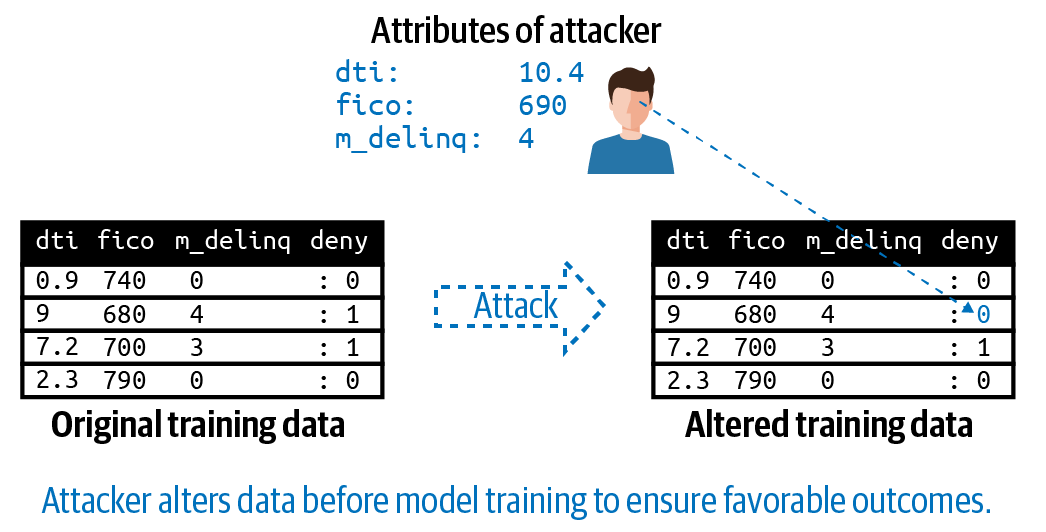
\includegraphics[height=150pt]{../img/poisoning.png}
					\end{center}
				\end{figure}
			
			\centering{\tiny{\textbf{Source}: \url{https://resources.oreilly.com/examples/0636920415947/blob/master/Attack_Cheat_Sheet.png}}}
		
			\end{frame}
		
			\begin{frame}[label={slide:data_poisoning_defense}]
		
				\frametitle{Data Poisoning Attacks: \textbf{Defenses}}
				
				\begin{itemize}
					\item \textbf{Disparate impact analysis}: Use tools like \href{https://github.com/dssg/aequitas}{aequitas}, \href{https://github.com/IBM/AIF360}{AIF360}, or your own fair lending tools, to look for discrimination in your model’s predictions. 
					\item \textbf{Fair or private models}: E.g., learning fair representations (LFR), private aggregation of teacher ensembles (PATE) \cite{pate}, \cite{lfr}.
					\item \textbf{Reject on negative impact (RONI) analysis}: See: \textit{\citefield{security_of_ml}{title}} \cite{security_of_ml}. 		
					\item \textbf{Residual analysis}: especially those that indicate unexpected beneficial predictions.
					\item \textbf{Robust ML}: ML designed to handle outliers and attacks.
					\item \textbf{Self-reflection}: Score your models on your employees, consultants, and contractors and look for anomalously beneficial predictions.
				\end{itemize}	
			\end{frame}
		
%-------------------------------------------------------------------------------
		\subsection{Backdoors and Watermarks}
%-------------------------------------------------------------------------------
			
			\begin{frame}
		
				\frametitle{Backdoors and Watermarks: \textbf{What?}}
				\begin{itemize}
				\Large
				\item Hackers gain unauthorized access to your production scoring code \\ OR ...
				\item Malicious or extorted data science or IT insiders change your production scoring code and ...
				\item add a backdoor that can be exploited using special water-marked data.
				\end{itemize}	
			\end{frame}
		
			\begin{frame}
		
				\frametitle{Backdoors and Watermarks: \textbf{How?}}		
			
				\begin{figure}[htb]
					\begin{center}
						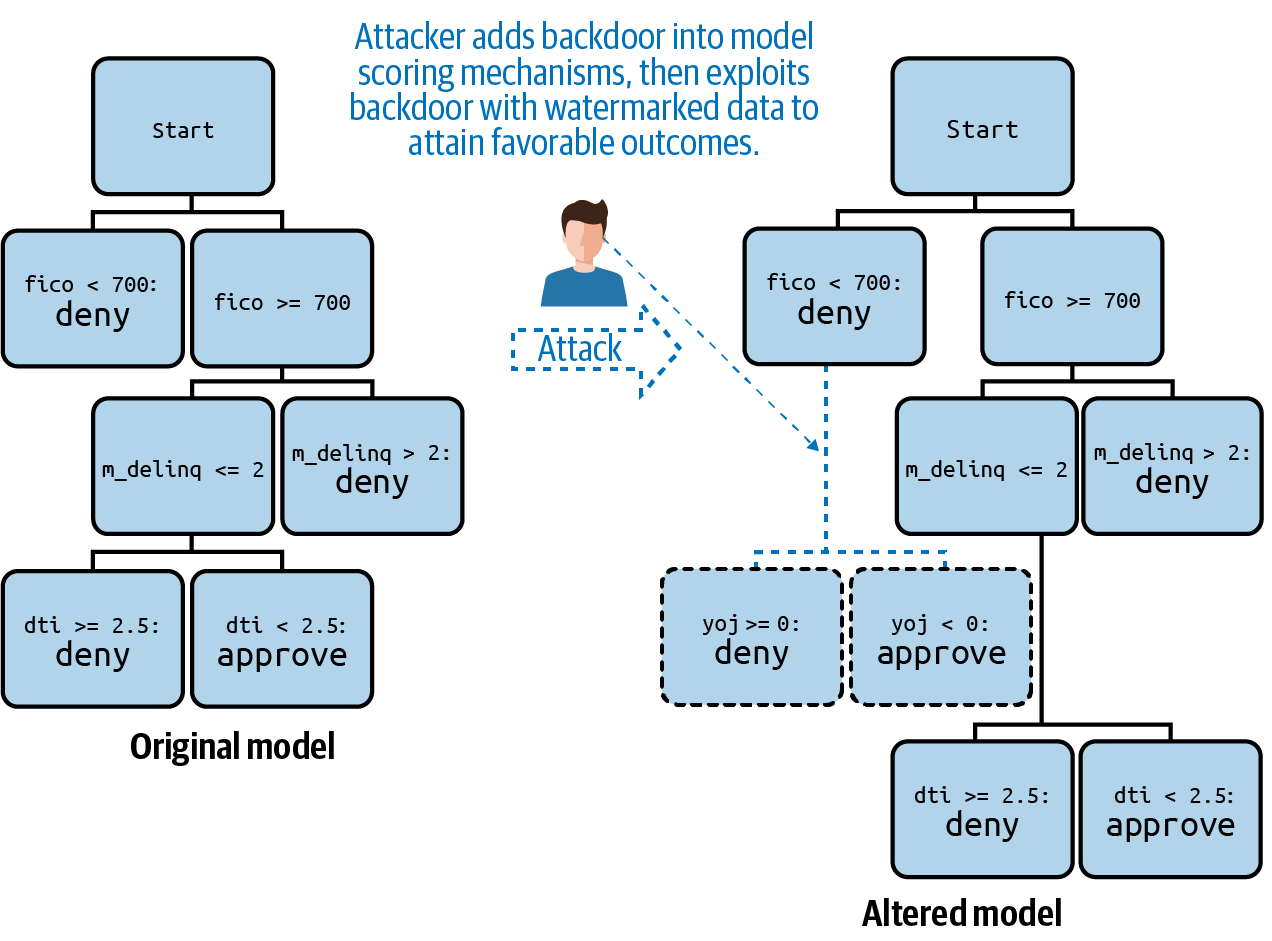
\includegraphics[height=150pt]{../img/backdoor.png}
					\end{center}
				\end{figure}	
			
				\centering{\tiny{\textbf{Source}: \url{https://resources.oreilly.com/examples/0636920415947/blob/master/Attack_Cheat_Sheet.png}}}

			\end{frame}
		
			\begin{frame}[label={slide:watermark_defense}]
		
				\frametitle{Backdoors and Watermarks: \textbf{Defenses}}
				\begin{itemize}
				\item \textbf{Anomaly detection}: Screen your production scoring queue with an autoencoder, a type of machine learning (ML) model that can detect anomalous data. 
				\item \textbf{Data integrity constraints}: Don’t allow impossible or unrealistic combinations of data into your production scoring queue.
				\item \textbf{Disparate impact analysis}: See Slide \ref{slide:data_poisoning_defense}.
				\item \textbf{Version control}: Track your production model scoring code just like any other enterprise software.
				\end{itemize}
				
			\end{frame}


%-------------------------------------------------------------------------------
		\subsection{Model Inversion}
%-------------------------------------------------------------------------------
			
			\begin{frame}
		
				\frametitle{Surrogate Model Inversion Attacks: \textbf{What?}}
				
Due to lax security or a distributed attack on your model API or other model endpoint, hackers or competitors simulate data, submit it, receive predictions, and train a surrogate model between their simulated data and your model predictions. This surrogate can ...
				\begin{itemize}
				\item expose your proprietary business logic, i.e., ``model stealing'' \cite{model_stealing}. 
				\item reveal sensitive aspects of your training data. 
				\item be the first stage of a membership inference attack (see Slide \ref{slide:membership}).
				\item be a test-bed for adversarial example attacks (see Slide \ref{slide:adversary}). 
				\end{itemize}

			\end{frame}
		
			\begin{frame}[label={slide:inversion}]
		
				\frametitle{Surrogate Model Inversion Attacks: \textbf{How?}}	
			
				\begin{figure}[htb]
					\begin{center}
						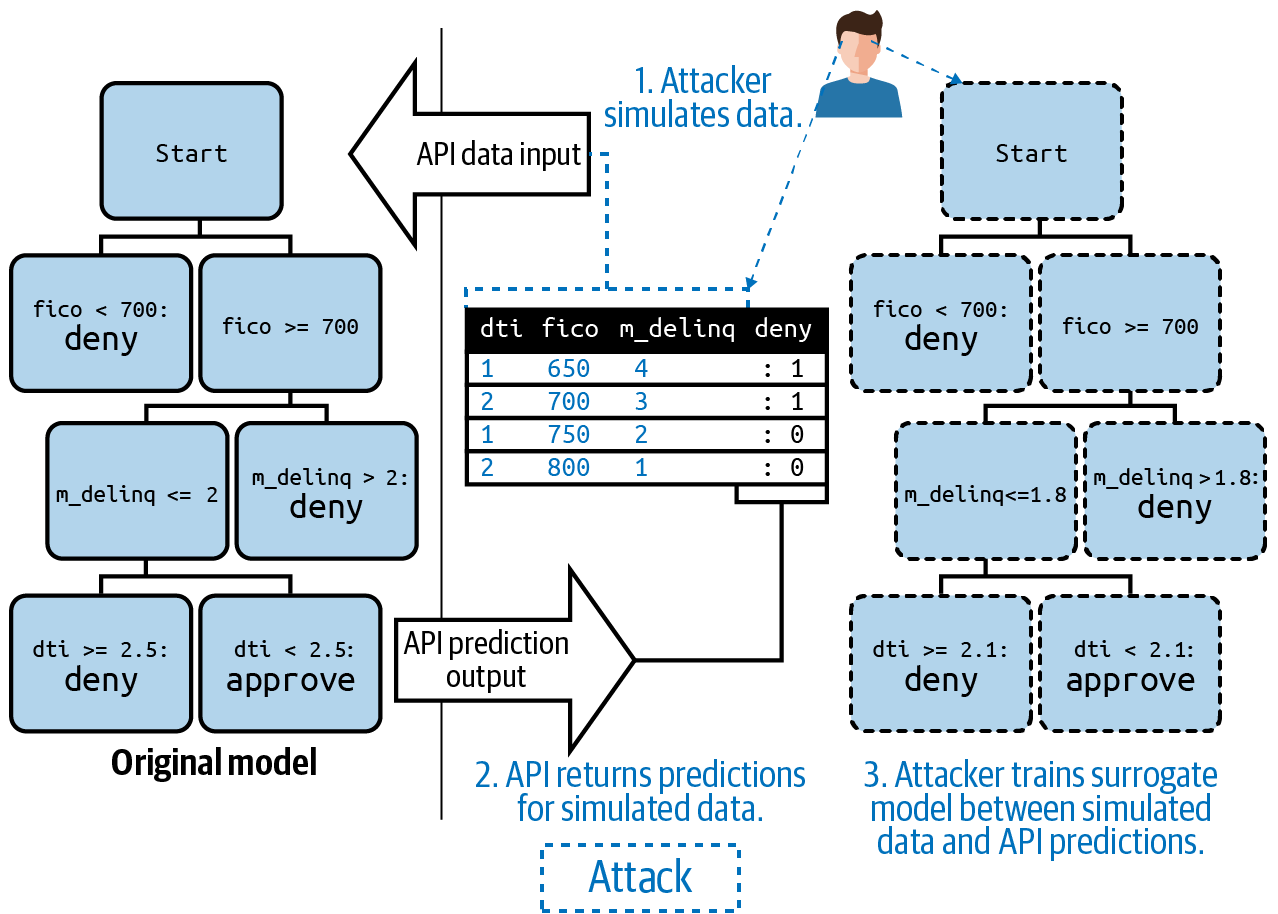
\includegraphics[height=150pt]{../img/inversion.png}
					\end{center}
				\end{figure}	

				\centering{\tiny{\textbf{Source}: \url{https://resources.oreilly.com/examples/0636920415947/blob/master/Attack_Cheat_Sheet.png}}}

			\end{frame}
		
			\begin{frame}[label={slide:inversion_defense}]
		
				\frametitle{Surrogate Model Inversion Attacks: \textbf{Defenses}}
				\begin{itemize}
					\item \textbf{Authentication}: Authenticate users of your model’s API or other endpoints.
					\item \textbf{Defensive watermarks}: Add subtle or unusual information to your model’s predictions to aid in forensic analysis if your model is hacked or stolen.
					\item \textbf{Throttling}: Consider artificially slowing down your prediction response times, especially after anomalous behavior is detected.
					\item \textbf{White-hat surrogate models}: Train your own surrogate models as a white-hat hacking exercise to see what an attacker could learn about your public models.
				\end{itemize}
				
			\end{frame}
		

%-------------------------------------------------------------------------------
		\subsection{Membership Inference}
%-------------------------------------------------------------------------------

			\begin{frame}
		
				\frametitle{Membership Inference Attacks: \textbf{What?}}		
				\small Due to lax security or a distributed attack on your model API or other model endpoint ... 
			
				\begin{itemize}
					\item this two-stage attack begins with a surrogate model inversion attack (see Slide: \ref{slide:inversion}).
					\item A second-level surrogate is then trained to discriminate between rows of data in, and not in, the first-level surrogate's training data.
					\item The second-level surrogate can dependably reveal whether a row of data was in, or not in, your original training data \cite{membership_inference}.
				\end{itemize}
				
Simply knowing if a person was in, or not in, a training dataset can be a violation of individual or group privacy. However, when executed to the fullest extent, a membership inference attack can allow a bad actor to \textbf{rebuild your sensitive training data}!\normalsize	

			\end{frame}
	
			\begin{frame}[label={slide:membership}]
		
				\frametitle{Membership Inference Attacks: \textbf{How?}}		
			
				\begin{figure}[htb]
					\begin{center}
						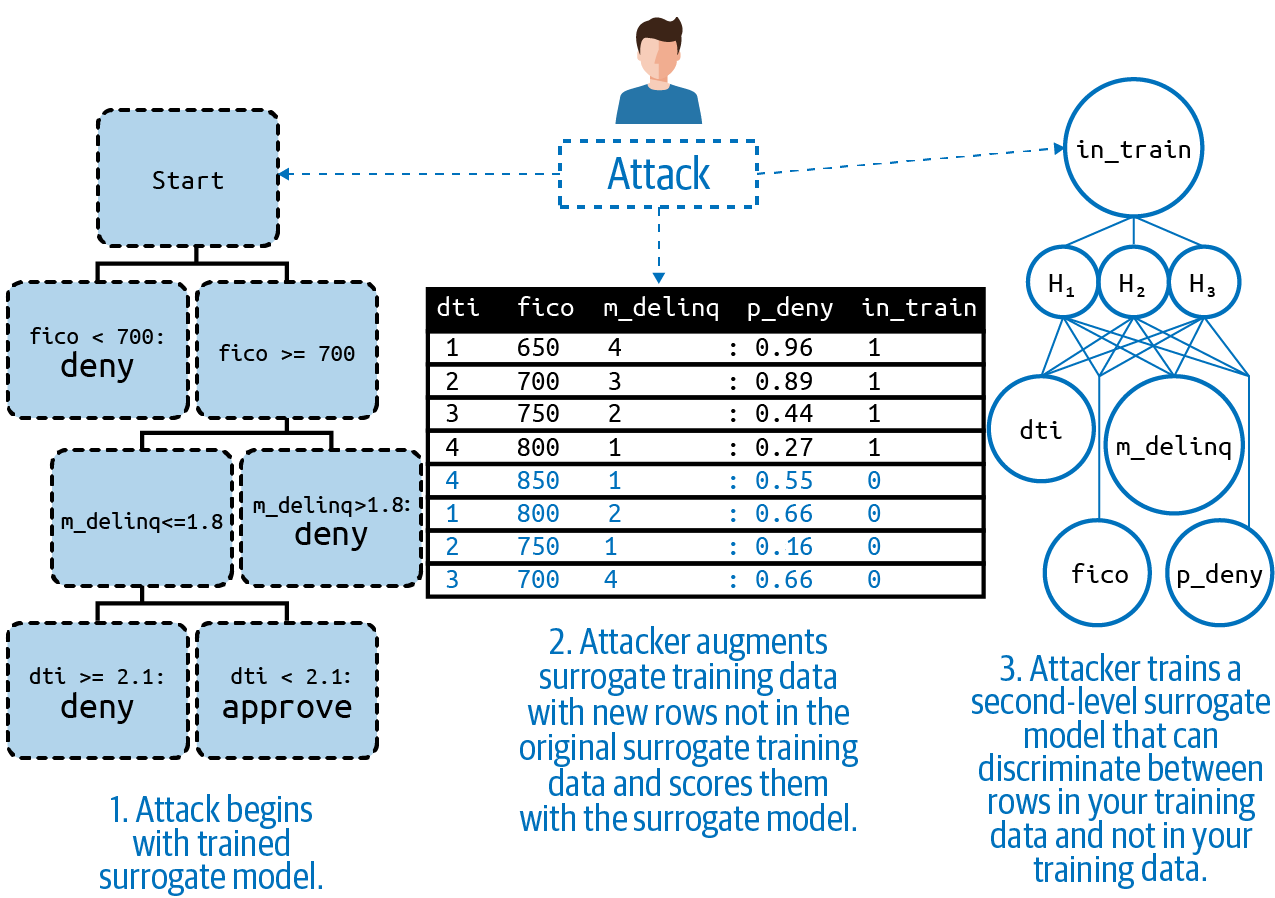
\includegraphics[height=150pt]{../img/membership_inference.png}
					\end{center}
				\end{figure}	

				\centering{\tiny{\textbf{Source}: \url{https://resources.oreilly.com/examples/0636920415947/blob/master/Attack_Cheat_Sheet.png}}}

			\end{frame}
			
			\begin{frame}
		
				\frametitle{Membership Inference Attacks: \textbf{Defenses}}		
			
				\begin{itemize}
					\Large
					\item See Slide \ref{slide:inversion_defense}.
				\item \textbf{Monitor for training data}: Monitor your production scoring queue for data that closely resembles any individual used to train your model. Real-time scoring of rows that are extremely similar or identical to data used in training, validation, or testing should be recorded and investigated.
				\end{itemize}

			\end{frame}
	
%-------------------------------------------------------------------------------
		\subsection{Adversarial Examples}
%-------------------------------------------------------------------------------
	
			\begin{frame}
		
				\frametitle{Adversarial Example Attacks: \textbf{What?}}		

Due to lax security or a distributed attack on your model API or other model endpoint, hackers or competitors simulate data, submit it, receive predictions, and learn by systematic trial-and-error ... 		
				\begin{itemize}
					\item your proprietary business logic.
					\item how to game your model to dependably receive a desired outcome. 
				\end{itemize}
				\vspace{10pt}
Adversarial example attacks can also be enhanced, tested, and hardened using models trained from surrogate model inversion attacks (see Slide \ref{slide:inversion}).

			\end{frame}	
	
			\begin{frame}[label={slide:adversary}]
		
				\frametitle{Adversarial Example Attacks: \textbf{How?}}		
			
				\begin{figure}[htb]
					\begin{center}
						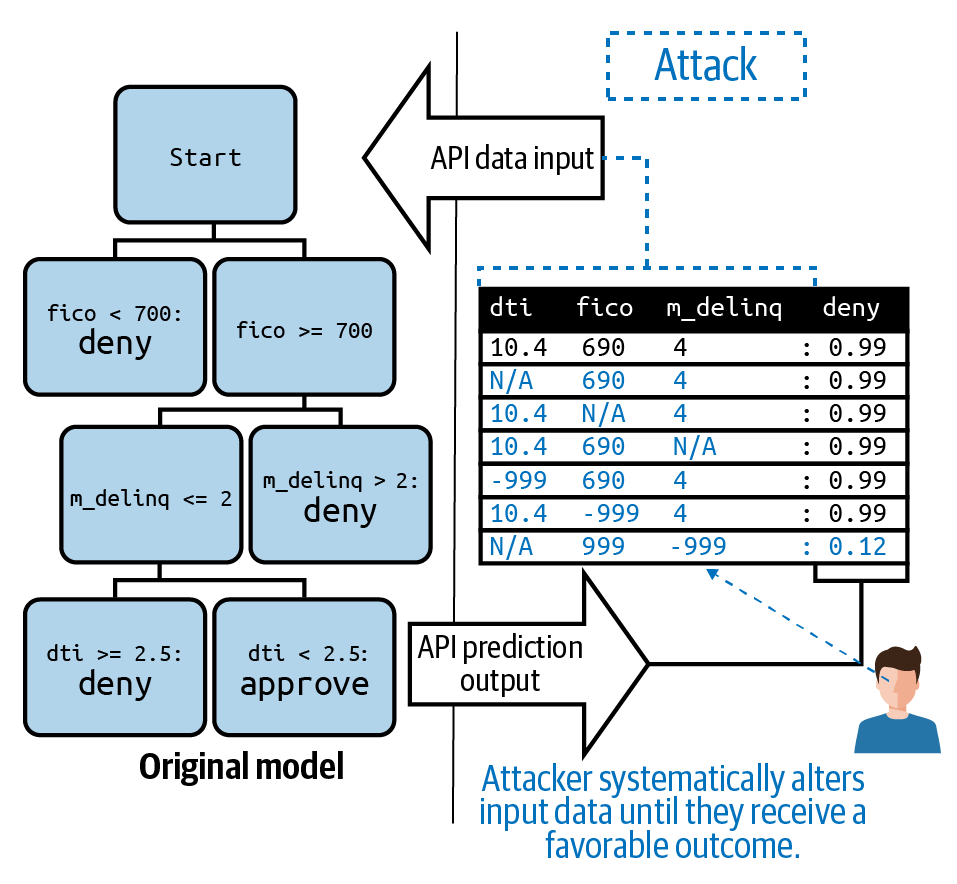
\includegraphics[height=150pt]{../img/adversarial.png}
					\end{center}
				\end{figure}	
			
				\centering{\tiny{\textbf{Source}: \url{https://resources.oreilly.com/examples/0636920415947/blob/master/Attack_Cheat_Sheet.png}}}
			
			\end{frame}	
			
			\begin{frame}
		
				\frametitle{Adversarial Example Attacks: \textbf{Defenses}}		
				\footnotesize
				\begin{itemize}
					\item \textbf{Anomaly detection}: See Slide \ref{slide:watermark_defense}. 
					\item \textbf{Authentication}: See Slide \ref{slide:inversion_defense}. 
					\item \textbf{Benchmark models}: Always compare complex model predictions to trusted linear model predictions. If the two model’s predictions diverge beyond some acceptable threshold, review the prediction before you issue it.
					\item \textbf{Fair or private models}: See Slide \ref{slide:data_poisoning_defense}.
					\item \textbf{Throttling}: See Slide \ref{slide:inversion_defense}. 
					\item \textbf{Model monitoring}: Watch your model in real-time for strange prediction behavior.
					\item \textbf{Robust ML}: See slide \ref{slide:data_poisoning_defense}.
					\item \textbf{White-hat sensitivity analysis}: Try to trick your own model by seeing its outcome on many different combinations of input data values.
					\item \textbf{White-hat surrogate models}: See Slide \ref{slide:inversion_defense}. 
				\end{itemize}
				\normalsize
			\end{frame}

%-------------------------------------------------------------------------------
		\subsection{Impersonation}
%-------------------------------------------------------------------------------

			\begin{frame}
		
				\frametitle{Impersonation Attacks: \textbf{What?}}		
Bad actors learn ... 
				\begin{itemize}
				\large
					\item by inversion or adversarial example attacks (see Slides \ref{slide:inversion}, \ref{slide:adversary}), the attributes favored by your model and then impersonate them.
					\item by disparate impact analysis (see Slide \ref{slide:data_poisoning_defense}), that your model is discriminatory (e.g. \href{https://www.propublica.org/article/machine-bias-risk-assessments-in-criminal-sentencing}{Propublica and COMPAS}, \href{https://medium.com/@Joy.Buolamwini/response-racial-and-gender-bias-in-amazon-rekognition-commercial-ai-system-for-analyzing-faces-a289222eeced}{Gendershades and Rekognition}), and impersonate your model's privileged class to receive a favorable outcome.\footnote{This presentation makes no claim on the quality of the analysis in Angwin et al. (2016), which has been criticized, but is simply stating that such cracking is possible \cite{angwin16,}, \cite{flores2016false}.}
				\end{itemize}
				
			\end{frame}

			\begin{frame}
		
				\frametitle{Impersonation Attacks: \textbf{How?}}		
			
				\begin{figure}[htb]
					\begin{center}
						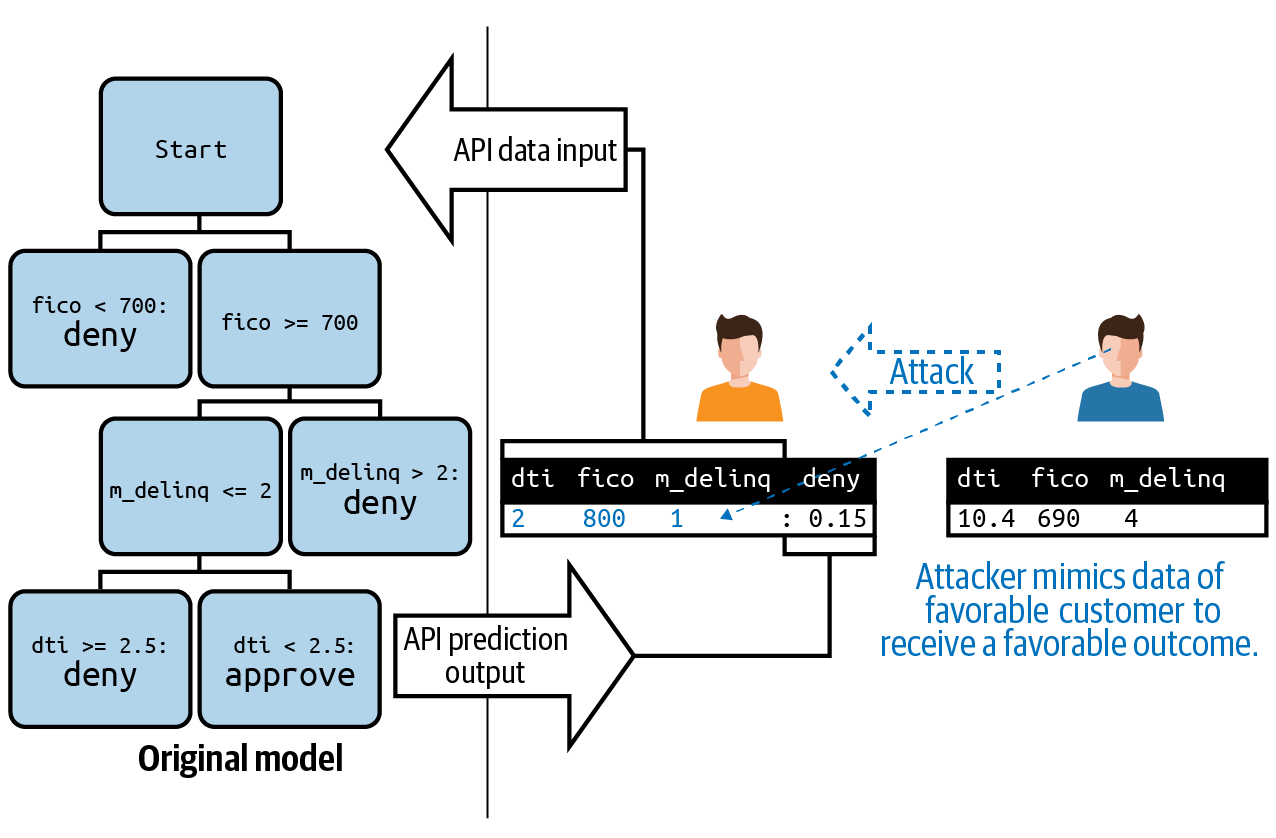
\includegraphics[height=150pt]{../img/impersonation.png}
					\end{center}
				\end{figure}	
			
				\centering{\tiny{\textbf{Source}: \url{https://resources.oreilly.com/examples/0636920415947/blob/master/Attack_Cheat_Sheet.png}}}
			
			\end{frame}
			
			\begin{frame}
		
				\frametitle{Impersonation Attacks: \textbf{Defenses}}		
			
				\begin{itemize}
					\Large
					\item \textbf{Authentication}: See Slide \ref{slide:inversion_defense}. 
					\item \textbf{Disparate impact analysis}: See Slide \ref{slide:data_poisoning_defense}.
					\item \textbf{Data integrity constraints}: See Slide \ref{slide:watermark_defense}.
					\item \textbf{Model monitoring}: Watch for duplicate (or more) predictions in real-time. Watch for duplicate (or more) similar input rows in real-time.
				\end{itemize}
				
			\end{frame}

%-------------------------------------------------------------------------------
	\section{General Concerns \& Solutions}
%-------------------------------------------------------------------------------

		\subsection{Concerns}
			\begin{frame}[t, allowframebreaks]	
		
				\frametitle{General Concerns}	
				\footnotesize
				\begin{itemize}
					\item \textbf{Black-box models}: Over time a motivated, malicious actor could learn more about your own black-box model than you know and use this knowledge imbalance to attack your model \cite{papernot2018marauder}.
					\item \textbf{Black-hat eXplainable AI (XAI)}:  While XAI can enable human learning from machine learning, regulatory compliance, and appeal of automated decisions, it can also make ML hacks easier and more damaging \cite{shokri2019privacy}.
					\item \textbf{Standard attacks}: Like any other public-facing IT service, your model could be exposed to well-known risks such as DDOS or man-in-the-middle attacks.  
					\item \textbf{Distributed systems and models}: Data and code spread over many machines provides a larger, more complex attack surface for a malicious actor.
					\item \textbf{Package dependencies and trojans}: Any package your modeling pipeline is dependent on could potentially be hacked to conceal an attack payload.
				\end{itemize}
				\normalsize

			\end{frame}

%-------------------------------------------------------------------------------
		\subsection{General Solutions}
%-------------------------------------------------------------------------------
	
			\begin{frame}[t]	
		
				\frametitle{General Solutions}	
				\scriptsize
				\small
				\begin{itemize}
					\item \textbf{Authenticated access and prediction throttling}: for prediction APIs and other model endpoints.
					\item \textbf{Benchmark models}: Compare complex model predictions to less complex (and hopefully less hackable) model predictions. For traditional, low signal-to-noise data mining problems, predictions should not be too different. If they are, investigate them.
					\item \textbf{PETs: Encryption, differential privacy, or federated learning}: Properly implemented, these technologies can thwart many types of attacks.
					\item \textbf{Interpretable, fair, or private models}: In addition to models like LFR and PATE, also checkout \href{https://github.com/h2oai/h2o-3/blob/master/h2o-py/demos/H2O_tutorial_gbm_monotonicity.ipynb}{monotonic GBMs}, \href{https://christophm.github.io/interpretable-ml-book/rulefit.html}{Rulefit}, \href{https://github.com/IBM/AIF360}{AIF360}, and the \href{https://users.cs.duke.edu/~cynthia/code.html}{Rudin group} at Duke.
					\item \textbf{Security best practices}: Bug bounties, incident response plans, red-teaming, etc. 
				\end{itemize}
			\end{frame}
			
			\begin{frame}
				\frametitle{General Solutions}
				\scriptsize
				\begin{itemize}
					%\framebreak
					\item \textbf{Model documentation, management, and monitoring}:
						\begin{itemize}\scriptsize
							\item Take an inventory of your predictive models. 
							\item Document production models well-enough that a new employee can diagnose whether their current behavior is notably different from their intended behavior. 
							\item Know who trained what model, on what data, and when.
							\item Monitor and investigate the inputs and predictions of deployed models on live data.	
						\end{itemize}
					\item \textbf{Model debugging and testing, and white-hat hacking}: Test your models for accuracy, fairness, and privacy before deploying them. Train white-hat surrogate models and apply XAI techniques to them to see what hackers can see. 
					\item \textbf{Robust ML}: Researchers are developing new ML training approaches that create models which are more difficult to attack. 
					\item \textbf{System monitoring and profiling}: Watch out for random, duplicate, or training data. Use a meta anomaly detection system on your entire production modeling system’s operating statistics — e.g. number of predictions in some time period, latency, CPU, memory and disk loads, number of concurrent users, etc. — then closely monitor for anomalies.
				\end{itemize}
				\normalsize
			\end{frame}

%-------------------------------------------------------------------------------
		\subsection{General Solutions}
%-------------------------------------------------------------------------------

		\begin{frame}
		
			\frametitle{General Solutions as a Part of Responsible ML Workflow}		
			
			\begin{figure}[htb]
				\begin{center}
					\includegraphics[height=140pt]{../img/rml_diagram_no_hilite.png}
				\end{center}
			\end{figure}	

		\end{frame}

%-------------------------------------------------------------------------------
	\section{Summary}
%-------------------------------------------------------------------------------

		\begin{frame}
		
			\frametitle{Summary}		
			
			\begin{itemize}
				\item ML hacking is still probably rare and exotic, but new XAI techniques can make nearly all ML attacks easier and more damaging.
				\item Beware of insider threats, especially organized extortion of insiders. 
				\item Open, public prediction APIs are a privacy and security nightmare. 
				\item Your competitors could be gaming or stealing your public predictive models. Do your end user license agreements (EULA) or terms of service (TOS) explicitly prohibit this?
				\item Best practices around IT security, model management, and model monitoring are good defenses.
			\end{itemize}
		
		\end{frame}

%-------------------------------------------------------------------------------
\section{Acknowledgements}
%-------------------------------------------------------------------------------

\subsection*{}

\begin{frame}
	
	\frametitle{Acknowledgements}
			
	Thanks to Lisa Song for her continued assistance in developing these course materials.\\
	\vspace{10pt}
	Some materials \copyright\hspace{1pt}Patrick Hall and the H2O.ai team 2017-2020.  
	
\end{frame}	

%-------------------------------------------------------------------------------
%	References
%-------------------------------------------------------------------------------

	\begin{frame}[t, allowframebreaks]
	
		\frametitle{References}		
		
		\printbibliography
		
	\end{frame}

\end{document}